%%%%%%%%%%%%%%%%%%%%%%%%%%%%%% -*- Mode: Latex -*- %%%%%%%%%%%%%%%%%%%%%%%%%%%%
%% 12-06.tex --      ICT4S Paper
%% Author          : Philip Johnson
%% Created On      : Mon Sep 23 11:52:28 2002
%% Last Modified By: Philip Johnson
%% Last Modified On: Fri Apr 16 15:19:50 2010
%%%%%%%%%%%%%%%%%%%%%%%%%%%%%%%%%%%%%%%%%%%%%%%%%%%%%%%%%%%%%%%%%%%%%%%%%%%%%%%
%%   Copyright (C) 2009 Philip Johnson
%%%%%%%%%%%%%%%%%%%%%%%%%%%%%%%%%%%%%%%%%%%%%%%%%%%%%%%%%%%%%%%%%%%%%%%%%%%%%%%
%% 

%% Home page:http://www.ict4s.org/

\documentclass{acm_proc_article-sp}
%\usepackage[final]{graphicx}
\usepackage{cite}
\usepackage{url}
% uncomment the % away on next line to produce the final camera-ready version
% and uncomment the \thispagestyle{empty} following \maketitle
%\pagestyle{empty}

\begin{document}

\title{Makahiki+WattDepot: An open source software stack for 
next generation energy research and education}
\subtitle{[Extended Abstract]}

\author{Philip M. Johnson\\
        Yongwen Xu\\
        Robert S. Brewer\\
        George E. Lee\\
        Andrea Connell\\
        Collaborative Software Development Laboratory\\
        Department of Information and Computer Sciences\\
        University of Hawai`i at M\=anoa\\
        Honolulu, HI 96822\\
        \{johnson, yxu, rbrewer, gelee, connell4\}@hawaii.edu\\
}


\maketitle

\section{Introduction}

Several characteristics of the traditional electrical energy infrastructure
of industrial societies have remained unchanged for almost 100 years.  First, energy
production has been centralized in power plants using ``firm'' energy sources such as coal, oil,
nuclear, or water.  Second, centralized production
has promoted centralized control of the grid, typically through a single or small number of
utilities with public regulation over their policies and rates.  Third, centralized
production and control has led to the predominence of ``macro-grids'', or grid
infrastructures designed to service hundreds of thousands to millions of
consumers. Finally, traditional grids have been designed to minimize the information about
energy required by consumers to utilize the service.  The typical consumer needs to know
almost nothing more than how to plug an appliance into an outlet, and can
assume that this exceedingly simple ``user interface'' will provide virtually unlimited
amounts of high quality energy at any time for a relatively small cost.

Unfortunately, the accelerating world-wide growth in demand for energy is
leading to a breakdown in this approach to electrical energy infrastructure.  Petroleum
products such as coal and oil are nonrenewable, are no longer reliably inexpensive, and
have been found to have a variety of adverse environmental effects.  Nuclear energy, while
relatively ``clean'', has risks that have caused countries such as Japan and Germany to
discontinue use of this form of energy generation.  

Addressing these emergent problems has led to the conceptualization of a ``smart grid'',
where a variety of decentralized, intermittent, renewable energy sources (for example,
wind, solar, and wave) would provide most or all of the power required by small-scale
``micro-grids'' servicing hundreds to thousands of consumers. Such a ``smart
grid'' will require consumers to transition from passive to active participation in
maintaining efficient and effective use of the grid's electrical capabilities.  For
example, these ``smart consumers'' should be able to tailor their use of electrical energy
to the types and amount of energy available in the grid at any point in time; minimizing
the overall use of non-renewable resources as well as peak loads on the grid.

Satisfying the radically different requirements and operating assumptions of this next
generation grid requires new kinds of software that enable research and experimentation
into the ways that electrical energy production and consumption can be collected,
analyzed, visualized, and provided to consumers in a way that enables a transition from
passive to active participation.  Since 2009, we have been designing, implementing, and
evaluating an open source software ``stack'' to facilitate this research.  This software
stack consists of two custom systems called
WattDepot\footnote{http://wattdepot.googlecode.com} and
Makahiki\footnote{http://github.com/csdl/makahiki}, along with the open source components
they rely upon (Java, Restlet, Postgres, Python, Django, Memcache).

In the full version of this paper, we will detail the novel features of WattDepot and
Makahiki, our experiences using them for research and education, and additional ways they
can be used for next generation energy research and
education.  The remainder of this extended abstract briefly introduces WattDepot and
Makahiki and our research experiences to date.

\section{WattDepot in Brief}

Software for energy collection, storage, and analysis tends to come in two flavors that
support two ends of the scalability spectrum.  At one end are utility-scale SCADA systems
and protocols which are intended to manage macro-grid data
\cite{SmartEnergy2.0,OSHAN,OpenPDC}.  At the other end are ``personal scale'' systems such
as those provided by energy meter or solar panel manufacturers which are intended to
manage information about single households \cite{TED,EMS100}.  We designed WattDepot to
support a middle ground that we refer to as ``enterprise-level'' energy management, in
which data concerning energy production and consumption of hundreds to thousands of
households can be usefully managed.  Figure \ref{fig:wattdepot} illustrates the
architecture of the system, where WattDepot sensors send data from meters attached to
energy devices to a server, which can then be queried by clients to provide visualizations
and analyses.

\begin{figure}
\begin{center}
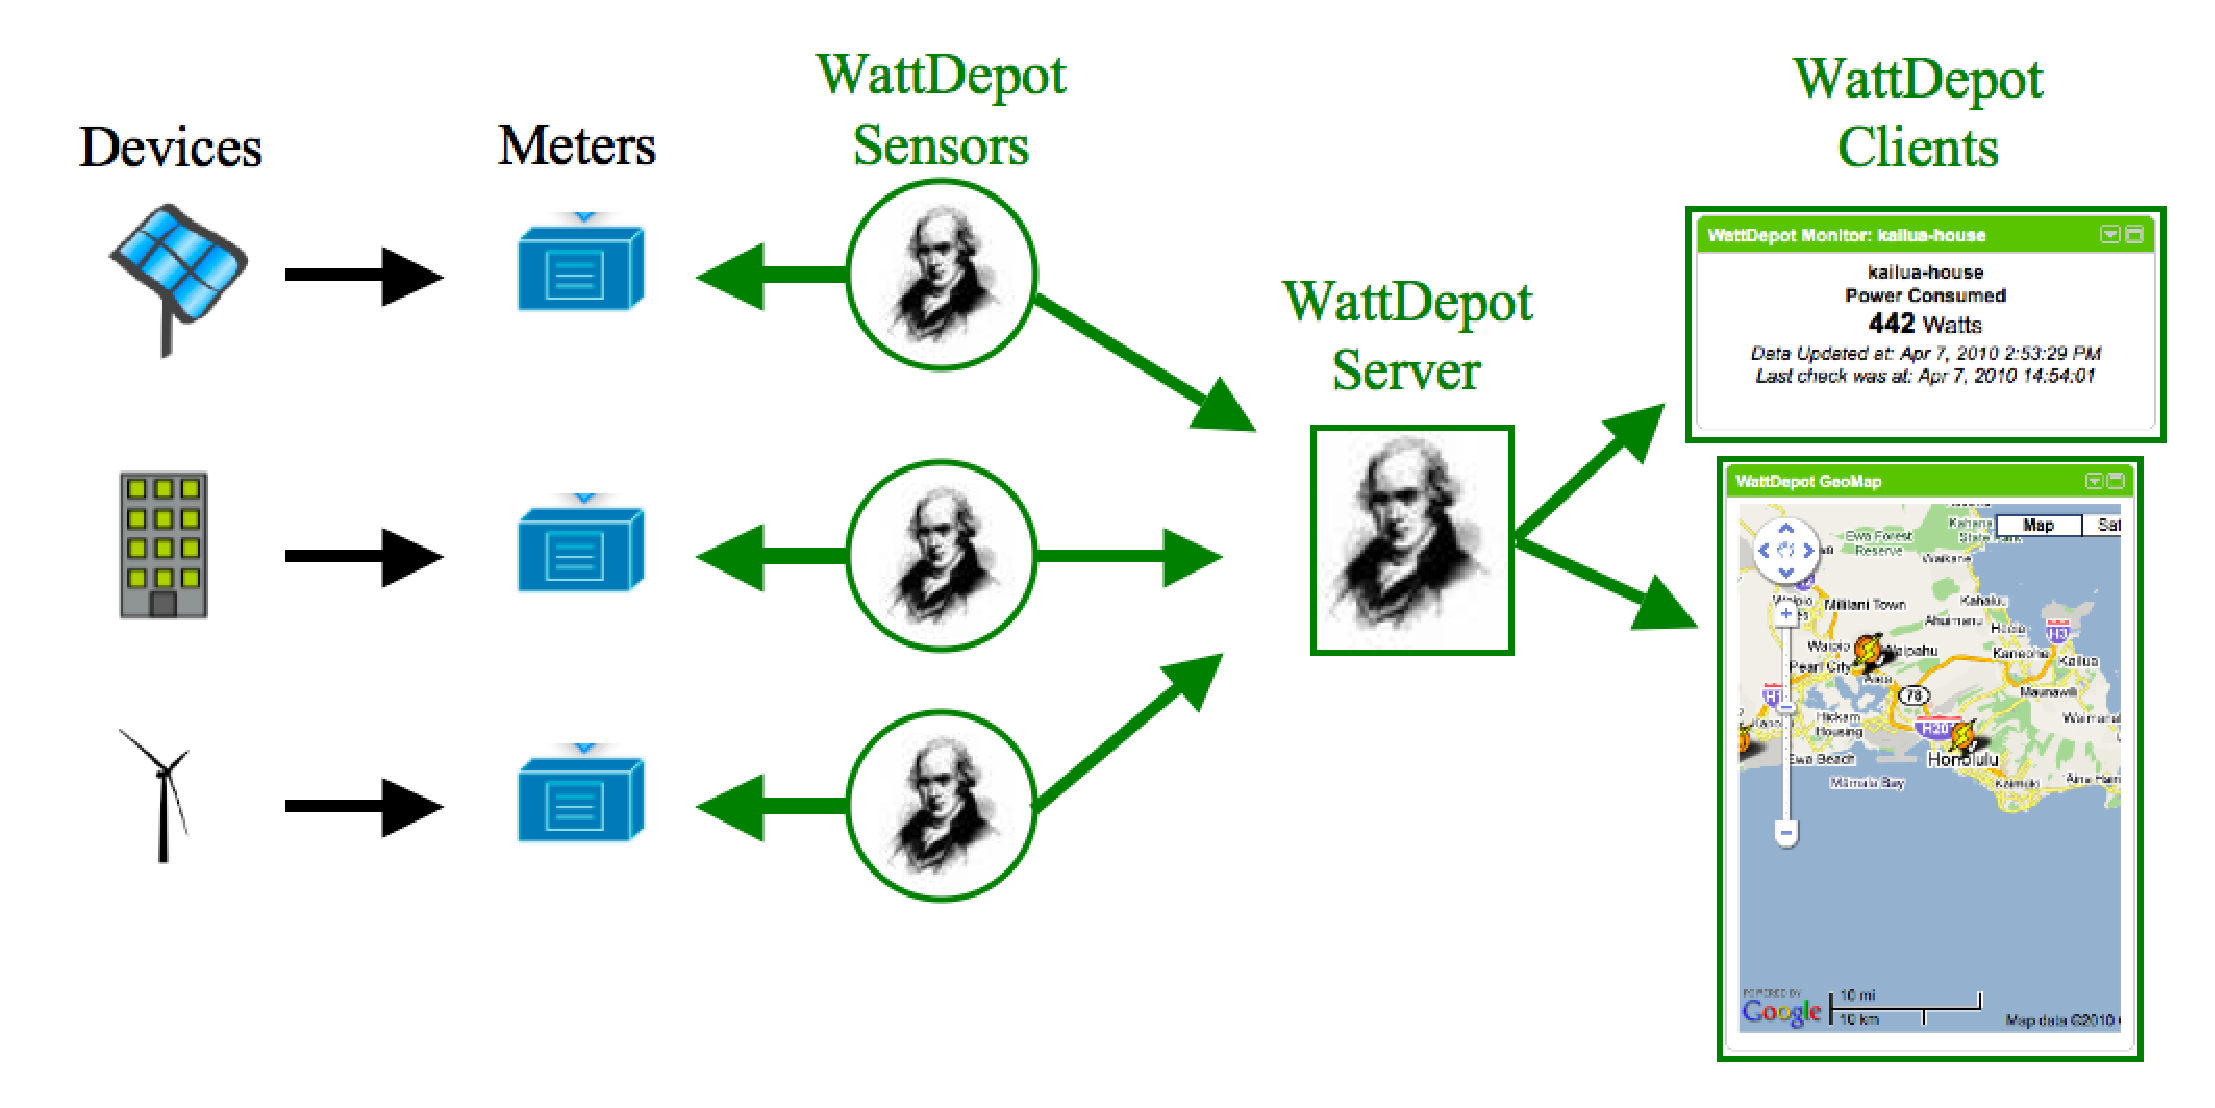
\epsfig{file=wattdepot-architecture, width=3in}
\end{center}
\caption{Architecture of WattDepot}
\label{fig:wattdepot}
\end{figure}

Our use of WattDepot has led to a novel set of capabilities to support
this middle ground.

First, unlike personal-scale systems that are typically tied to a particular
manufacturer's product, WattDepot is agnostic about the kinds of meters used to monitor
energy production and consumption data, and whether the data is personal-scale or
utility-scale. It provides a REST protocol for data transmission that can be used to
implement clients for a wide variety of devices; the major constraint is that these
devices need to have Internet access. WattDepot clients can be written in any language
that supports the HTTP protocol. We provide a high-level client library for Java.

Second, WattDepot can represent aggregations of power sou\-rces. For example, a building
might have multiple meters monitoring energy consumption, one per floor. WattDepot can
represent the power consumed by individual floors, as well as an aggregate source
representing the building as a whole. Aggregations can be nested, so that floors can be
aggregated into buildings, buildings into neighborhoods, and neighborhoods into cities.

Third, WattDepot automatically performs data interpolation when necessary. For example, a
meter might provide a snapshot of energy usage once per hour for a given device. Clients
can request the power consumed by this device at any time instant, and WattDepot will
automatically provide interpolation when the requested time does not match a time for
which actual sensor data is available.

Fourth, WattDepot is architecturally decoupled from the underlying data storage
technology. This supports experimentation with both traditional relational as well as
NoSQL technologies, and facilitates scalability. Currently, WattDepot implements support
for Derby, Postgres, and BerkeleyDB storage systems.

Fifth, WattDepot is designed to support both PaaS and local installation. We have deployed
WattDepot to the Heroku cloud-based hosting service.

Sixth, WattDepot implements support for "ephemeral" data. In some application scenarios,
it is useful to send energy data to the WattDepot server quite frequently (i.e. every few
seconds) so that clients can monitor current energy consumption with low latency. However,
that rate of data sampling is not necessary for historical analyses, which may only
require energy data sampling at the rate of every few minutes. WattDepot supports this
situation through "ephemeral" data, which creates an in-memory "window" during which all
recently received energy data is available for retrieval, but stored in the repository
only at a much lower sampling rate.

Seventh, WattDepot can be effectively used for simulation and what-if scenario
development, as well as for management of live energy data.  This makes it appropriate as
a kind of technological ``scaffolding'' for smart grid applications, where WattDepot can
provide clients with simulated production and consumption data early in development, with
the simulated data transitioning to live data as these sources go online later in development.

\section{Makahiki in Brief}

The feature set of WattDepot creates attractive infrastructure for management of energy
data, but research suggests that effective participation of consumers in a next generation
smart grid requires more than simple feedback to consumers about their consumption,
particularly given the passive nature of their involvement for the past 100 years. 

The second component of our open source software stack, Makahiki, represents research
intended to create synergy between the need to create knowledge and engagement regarding
energy and the ability of so-called ``serious game'' techniques and/or energy feedback to
create participation and engagement \cite{Deterding2011mt,darby-review-2006,Faruqui09,petersen-dorm-energy-reduction}.
In Makahiki, online world game mechanics are employed with the goal of affecting
real-world energy behaviors.  The ultimate goal is to not just affect energy behaviors
during the course of the game, but to produce long lasting, sustained change in energy
behaviors and outlooks by participants. Figure \ref{fig:makahiki-architecture} illustrates
the architecture of Makahiki.

\begin{figure}
\begin{center}
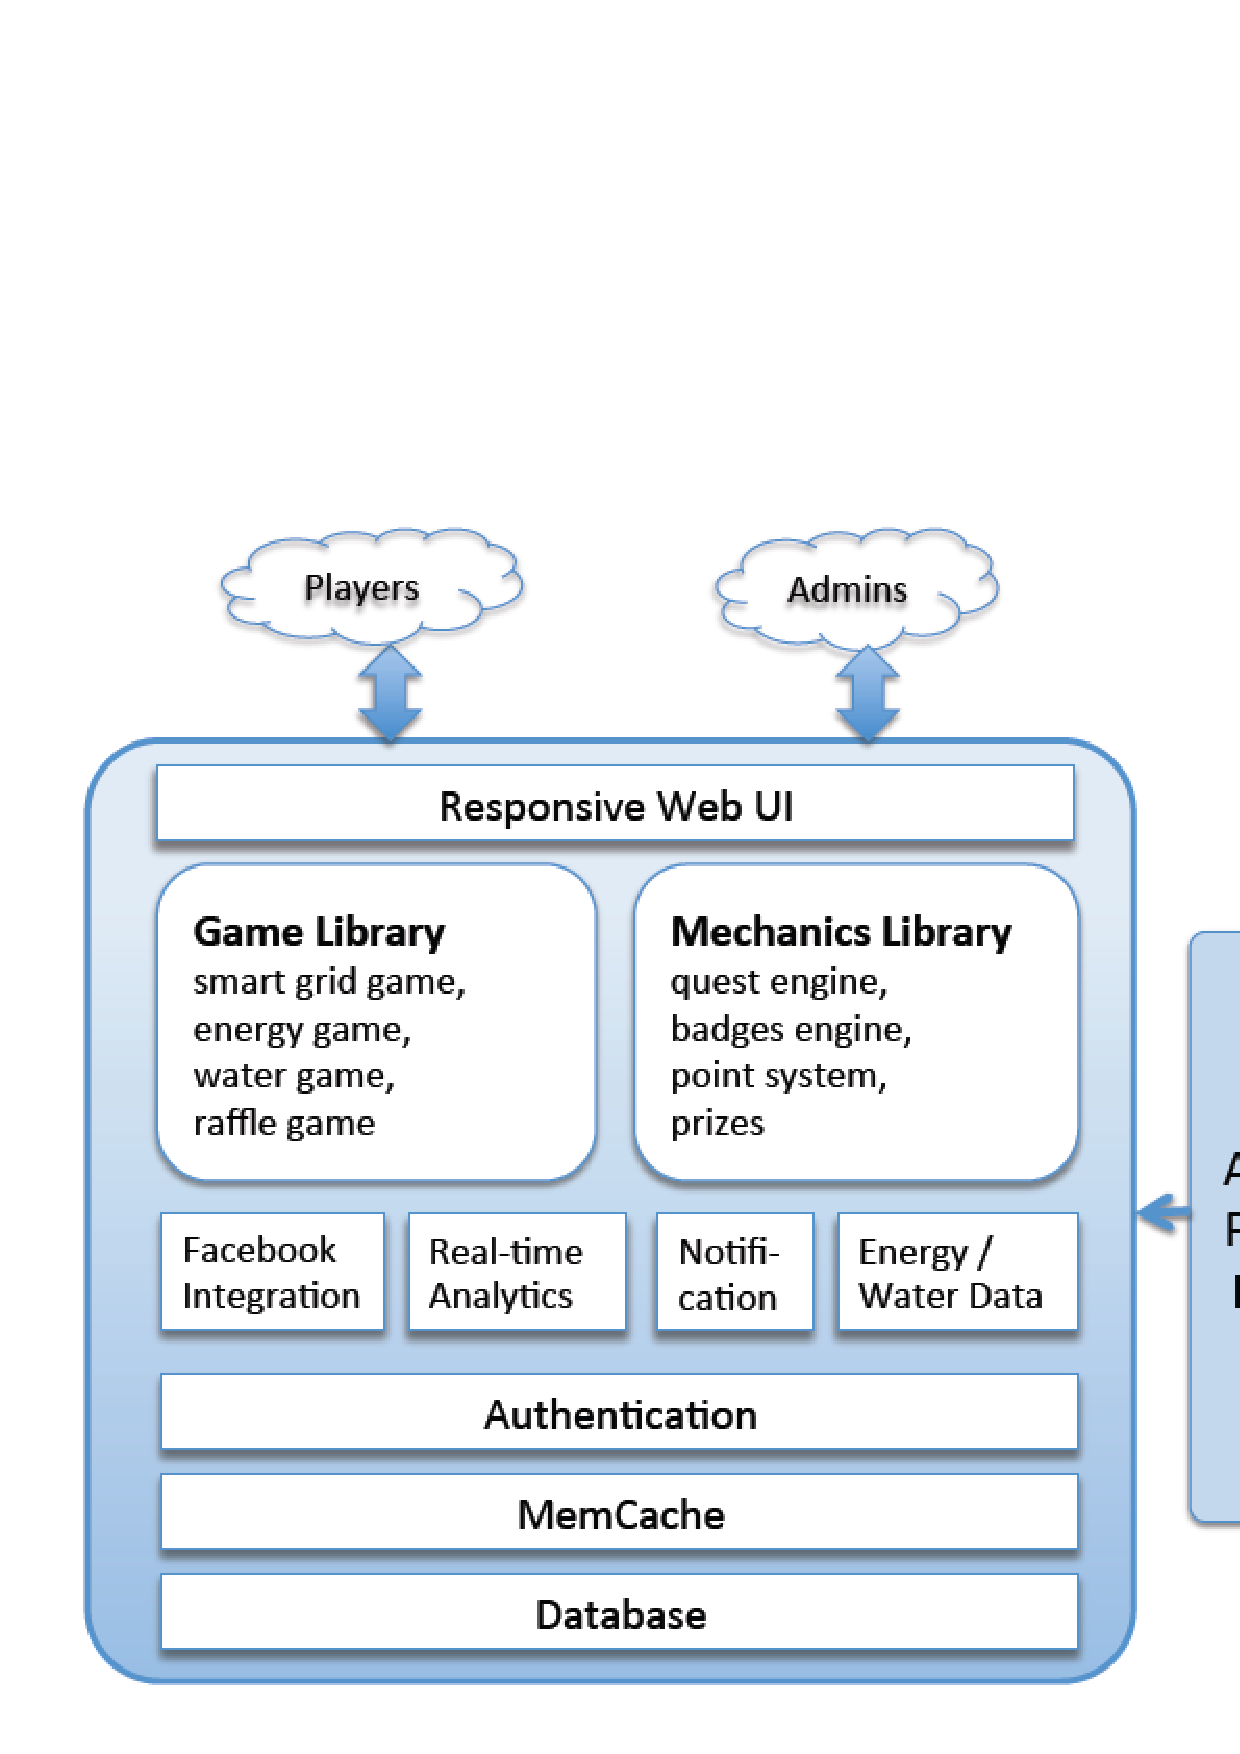
\epsfig{file=makahiki-system-architecture, width=3in}
\end{center}
\caption{Architecture of Makahiki}
\label{fig:makahiki-architecture}
\end{figure}

Makahiki consists of a configurable game engine that can be customized to the needs of
different organizations.  It includes a library of pre-built game ``widgets'' that
implement a variety of game mechanics.  Using the widgets, an organization can create an
custom energy challenge in which players can compete individually and/or in teams to earn
the most points by reducing their energy consumption as well as by learning about energy
concepts in general.  Some of the pre-built widgets include:

The {\em Smart Grid Game widget} is the primary place players go to learn about energy issues and earn
points.  The Smart Grid Game supports four different kinds of tasks: activities,
commitments, events, and excursions. 

The {\em Daily Energy Goal Game widget} provides a way for players to earn points by reducing their
current consumption from a baseline that is typically determined prior to the challenge.
Both the historical baseline data and the current consumption is typically provided
through calls by Makahiki to an underlying WattDepot server.

%% 1500 words here.

The {\em Raffle Game widget} provides a way to incentivize participation from all individuals, even
those who are not in the running for a top prize. For every 25 points a player earns, they
receive one virtual raffle ticket. Players can dynamically allocate their tickets to any
raffle prizes they are interested in at any time, up to the end of the raffle.

The {\em Social and Referral Bonus widgets} provide game mechanics that help encourage
participation by providing additional points to users who participate in activities with
other users and/or facilitate the entry of new users into an energy challenge. 

\section{Experiences in brief}

As a preliminary assessment of the Makahiki+WattDepot software stack, we designed and
implemented an energy challenge called the ``Ku\-kui Cup'' for over 1,000 first year
students living in the residence halls at the University of Hawaii in Fall, 2011.  We
installed 40 Shark 200-S meters throughout the residence halls, and used the ModBus
WattDepot sensors to gather instantaneous power and cumulative energy every 15 seconds.
Figure \ref{fig:golow} shows a portion of the Go Low page, which contains two widgets
(Power Meter and Daily Energy Goal Game) that are based upon WattDepot data.

\begin{figure}
\begin{center}
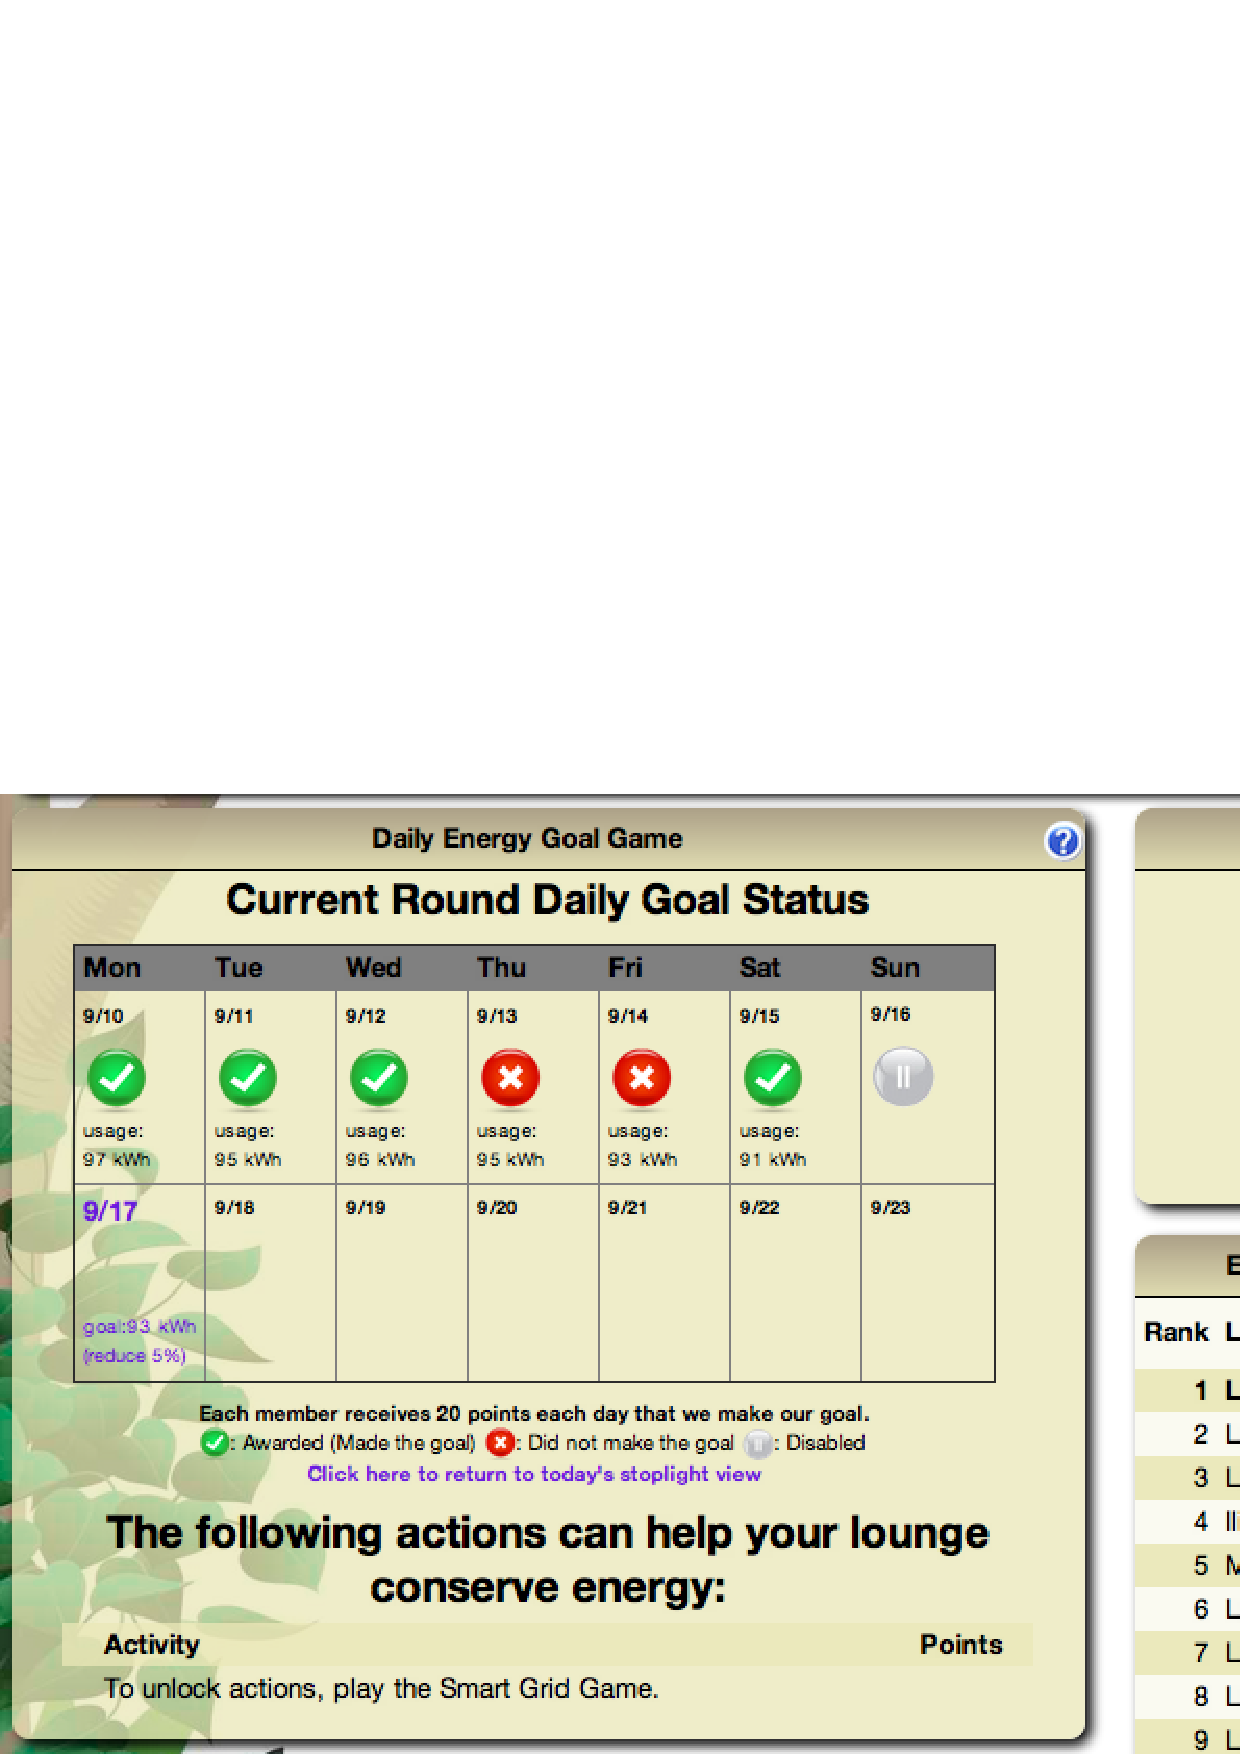
\epsfig{file=golow, width=3in}
\end{center}
\caption{An energy challenge implemented in Makahiki that visualizes WattDepot data}
\label{fig:golow}
\end{figure}

Response to this initial challenge was very positive.   Over 400 students participated,
for an adoption rate of approximately 40\%.  In a survey of those participating students
conducted near the end of the challenge, over 90\% of them said they would play the game
if it was offered next year.  60\% of participants said ``ease of use'' was the thing they
liked best about the website.  40\% responded ``Nothing'' when asked what was
confusing about the website, and 32\% responded ``Nothing'' when asked what they would
change about the website.  The survey did yield insights into what could be improved,
including the ability to introduce new games at points during the challenge, to provide
better access to other player data, and simplify navigation. 

The full version of this paper will go into more detail on our experiences as well as the
changes and enhancements we have made to the Makahiki+WattDepot software stack in
preparation for three energy challenges to be held in Fall, 2012.

\bibliographystyle{IEEEtran}
\bibliography{smartconsumer,csdl-trs,gamification,sustainability}


\end{document}
